\documentclass[14pt]{article}
\usepackage{amsmath}
\usepackage{amssymb,times}
\usepackage{graphicx}
\def\MM#1{\boldsymbol{#1}}

\title{How we do REXI}
\author{J. Shipton and C. J. Cotter}

\begin{document}
\maketitle
We are solving a system of the form

\begin{equation}
U(t) = \mathcal{L}U.
\end{equation}

Using an exponential integrator the solution of this system is

\begin{equation}
U(t) = e^{(t-t_0)\mathcal{L}}U(t_0).
\end{equation}

We compute the matrix exponential using the rational approximation

\begin{equation}
  e^{\tau\mathcal{L}}U(t_0) \approx \Sigma_{n=-N}^N\beta_n(\tau\mathcal{L} + \alpha_n)^{-1}U(t_0),
\end{equation}

\noindent where $\tau = t-t_0$, $\alpha_n$, and $\beta_n$ are complex
valued coefficiants given in Haut 2015, and computed using a python
version of Martin Schreiber's code.

For each $n$ we solve

\begin{equation}\label{neqn}
(\tau\mathcal{L} + \alpha_n)U_n = \beta_nU(t_0).
\end{equation}

For the linear shallow water system with constant $f$ we have

\begin{equation}
  \mathcal{L}U =
  \begin{pmatrix}
    -f\MM{u}^\perp - g\nabla h \\
    -H\nabla\cdot\MM{u}
  \end{pmatrix},
\end{equation}

\noindent so equation \ref{neqn} becomes

\begin{align}
  \tau(-f\MM{u_n}^\perp - g\nabla h_n) + \alpha_n\MM{u_n} &= \beta_n\MM{u_0}\\
  \tau(-H\nabla\cdot\MM{u_n}) + \alpha_nh_n &= \beta_nh_0
\end{align}

The weak form is

\begin{align}
  -\tau f\langle\MM{w}, \MM{u_n}^\perp\rangle + \tau g\langle\nabla\cdot\MM{w}, h_n\rangle + \alpha_n\langle\MM{w}, \MM{u_n}\rangle &= \beta_n\langle\MM{w}, \MM{u_0}\rangle \label{weak u}\\
  -\tau H\langle\phi, \nabla\cdot\MM{u_n}\rangle + \alpha_n\langle\phi, h_n\rangle &= \beta_n\langle\phi, h_0\rangle. \label{weak h}
\end{align}

Although $U(t_0)$ and the solution $U(t)$ are real valued, the complex
valued coefficients require that we work with complex numbers. Since
Firedrake does not yet have this capability, we write out the real and
imaginary components ourselves:

\begin{align}
  \MM{w} &= \MM{w}^r - i\MM{w}^i, \\
  \MM{u_n} &= \MM{u}_n^r + i\MM{u}_n^i
\end{align}

\noindent and likewise for $\phi$ and $h$ and the coeffiecients
$\alpha_n$ and $\beta_n$. Writing this out and equating real parts of
equations \ref{weak u}-\ref{weak h} gives

\begin{align}
  \begin{split}
    -\tau f\big(\langle\MM{w}^r, {\MM{u}_n^r}^\perp\rangle + \langle\MM{w}^i, {\MM{u}_n^i}^\perp\rangle\big) \\
  + \tau g\big(\langle\nabla\cdot\MM{w}^r, h_n^r\rangle + \langle\nabla\cdot\MM{w}^i, h_n^i\rangle\big) \\
  + \alpha_n^r(\langle\MM{w}^r, \MM{u}_n^r\rangle + \langle\MM{w}^i, \MM{u}_n^i\rangle) \\
  - \alpha_n^i(\langle\MM{w}^r, \MM{u}_n^i\rangle - \langle\MM{w}^i, \MM{u}_n^r\rangle) &= \beta_n^r\langle\MM{w}^r, \MM{u}_0\rangle + \beta_n^i\langle\MM{w}^i, \MM{u}_0\rangle
  \end{split}\\
  \begin{split}
    -\tau H \big(\langle\phi^r, \nabla\cdot\MM{u}_n^r\rangle + \langle\phi^i, \nabla\cdot\MM{u}_n^i\rangle\big) \\
    +\alpha_n^r\big(\langle\phi^r, h_n^r\rangle + \langle\phi^i, h_n^i\rangle\big) \\
    -\alpha_n^i\big(\langle\phi^r, h_n^i,\rangle - \langle\phi^i, h_n^r\rangle\big) &= \beta_n^r\langle\phi^r, h_n^r\rangle + \beta_n^i\langle\phi^i, h_n^i\rangle
  \end{split}
\end{align}

Reassuringly, if we return to equation \ref{neqn} and equate real and
imaginary parts before writing out the weak form, we obtain the same
answer, as follows:

\begin{align}
  (\tau\mathcal{L} + \alpha_n^r)U_n^r - \alpha_n^iU_n^i &= \beta_n^rU_0, \\
  (\tau\mathcal{L} + \alpha_n^r)U_n^i + \alpha_n^iU_n^r & = \beta_n^iU_0.
\end{align}

Now the weak form is

\begin{align}
  -\tau f\langle\MM{w}^r, {\MM{u}_n^r}^\perp\rangle + \tau g\langle\nabla\cdot\MM{w}^r, h_n^r\rangle + \alpha_n^r\langle\MM{w}^r, \MM{u}_n^r\rangle - \alpha_n^i\langle\MM{w}^r, \MM{u}_n^i\rangle &= \beta_n^r\langle\MM{w}^r, \MM{u}_0\rangle, \\
  -\tau H\langle\phi^r, \nabla\cdot\MM{u}_n^r\rangle + \alpha_n^r\langle\phi^r, h^r\rangle - \alpha_n^i\langle\phi^r, h_n^i\rangle & = \beta_n^r \langle\phi^r, h_0\rangle, \\
  -\tau f\langle\MM{w}^i, {\MM{u}_n^i}^\perp\rangle + \tau g\langle\nabla\cdot\MM{w}^i, h_n^i\rangle + \alpha_n^r\langle\MM{w}^i, \MM{u}_n^i\rangle + \alpha_n^i\langle\MM{w}^i, \MM{u}_n^r\rangle &= \beta_n^r\langle\MM{w}^i, \MM{u}_0\rangle, \\
  -\tau H\langle\phi^i, \nabla\cdot\MM{u}_n^i\rangle + \alpha_n^r\langle\phi^i, h^i\rangle + \alpha_n^i\langle\phi^i, h_n^r\rangle & = \beta_n^r \langle\phi^i, h_0\rangle,
\end{align}

\noindent as above.

\section{Results}

Below are some figures comparing results from the REXI solver to a
standard implicit midpoint timestepping scheme. These were obtained
using a spatial resolution of $128\times 128$ and with the REXI
parameters $h=0.2$ and $M=256$. The initial condition is the wave
scenario in Martin's 2016 paper and the fields are plotted at
$t=0.1$. For the implicit midpoint solver $dt=0.001$ and for REXI
$\tau=0.1$. These parameters should result in an error of around
$10^{-4}$.

Note that the agreement between the figures looks great (now that we're recreating the solver for each $n$)!

\begin{figure}
  \centering
  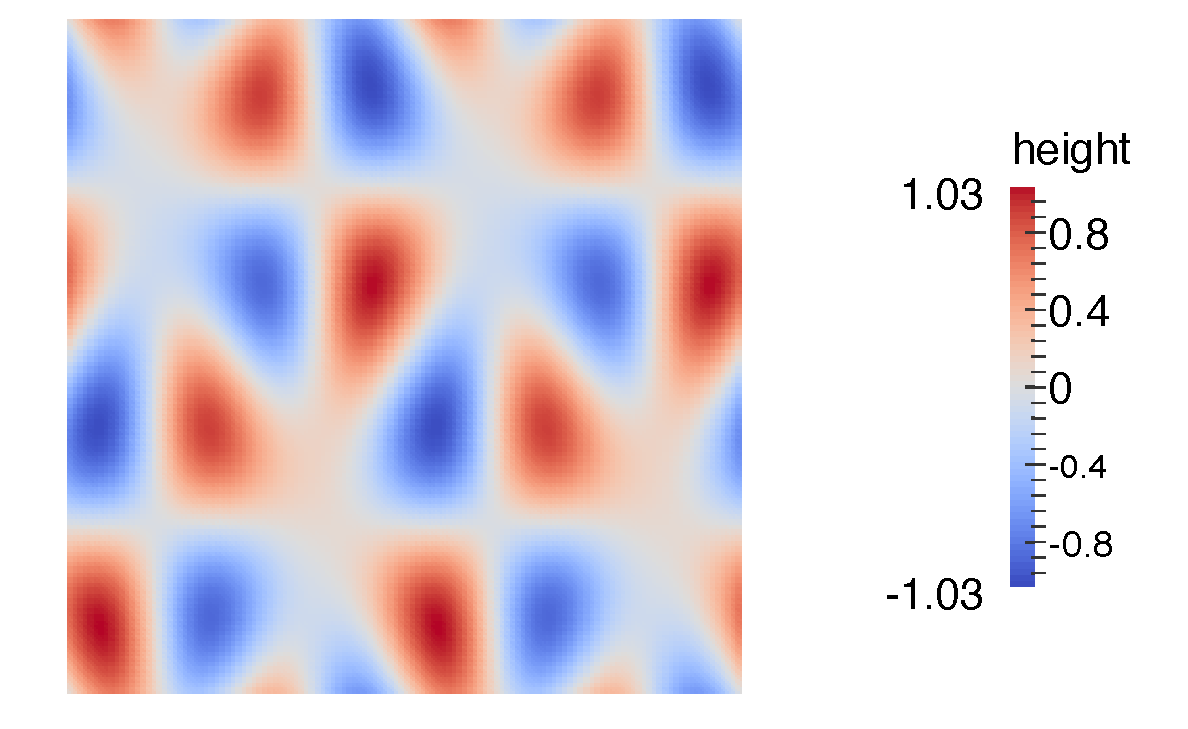
\includegraphics[width=0.45\textwidth]{results/t0.1/IM_h}
  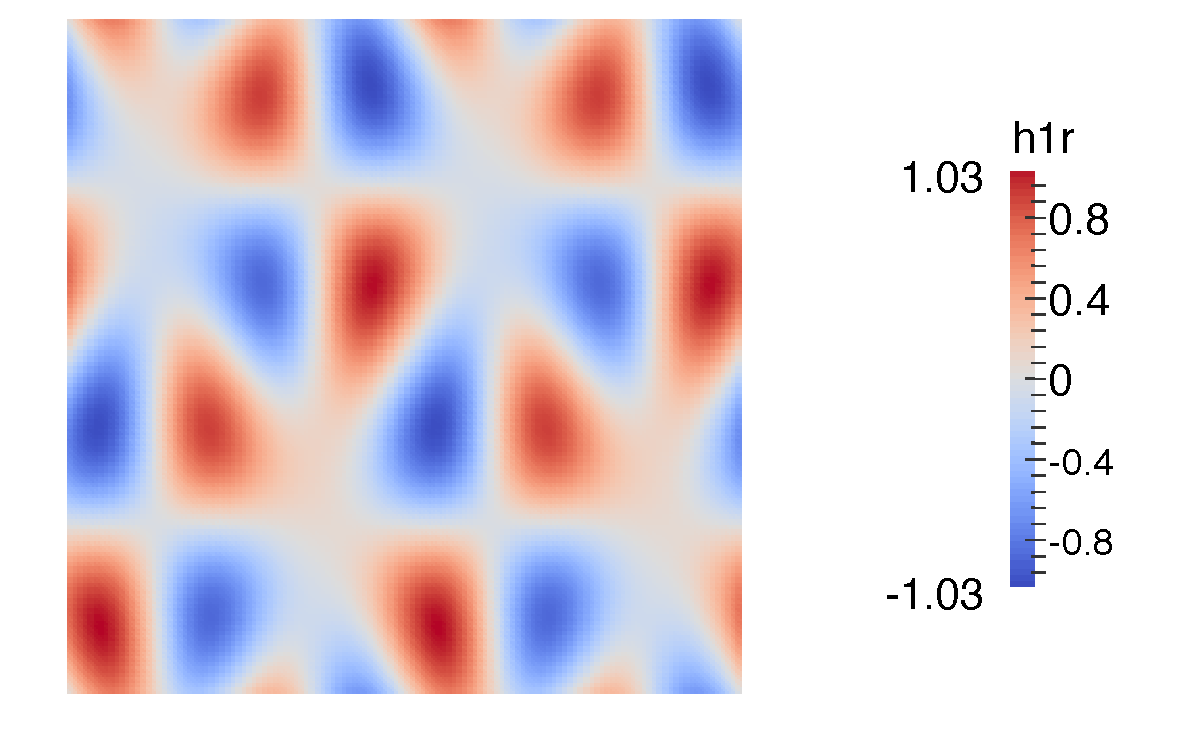
\includegraphics[width=0.45\textwidth]{results/t0.1/rexi_h}\\
  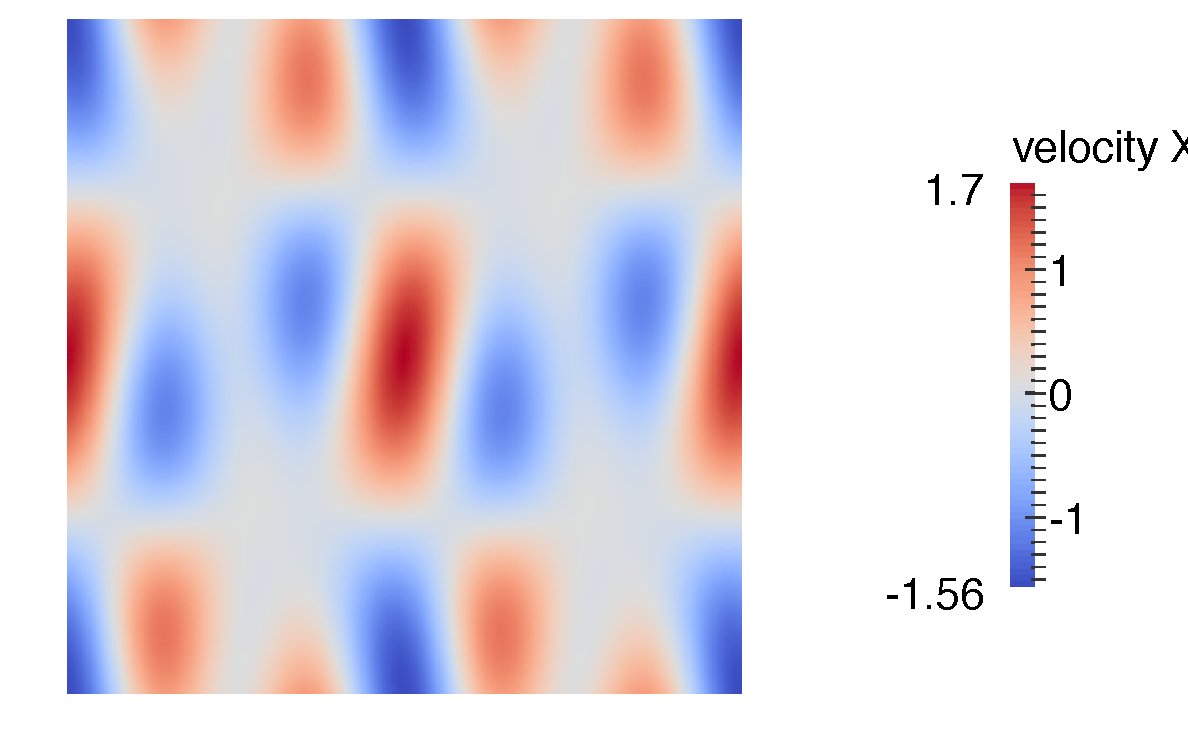
\includegraphics[width=0.45\textwidth]{results/t0.1/IM_u}
  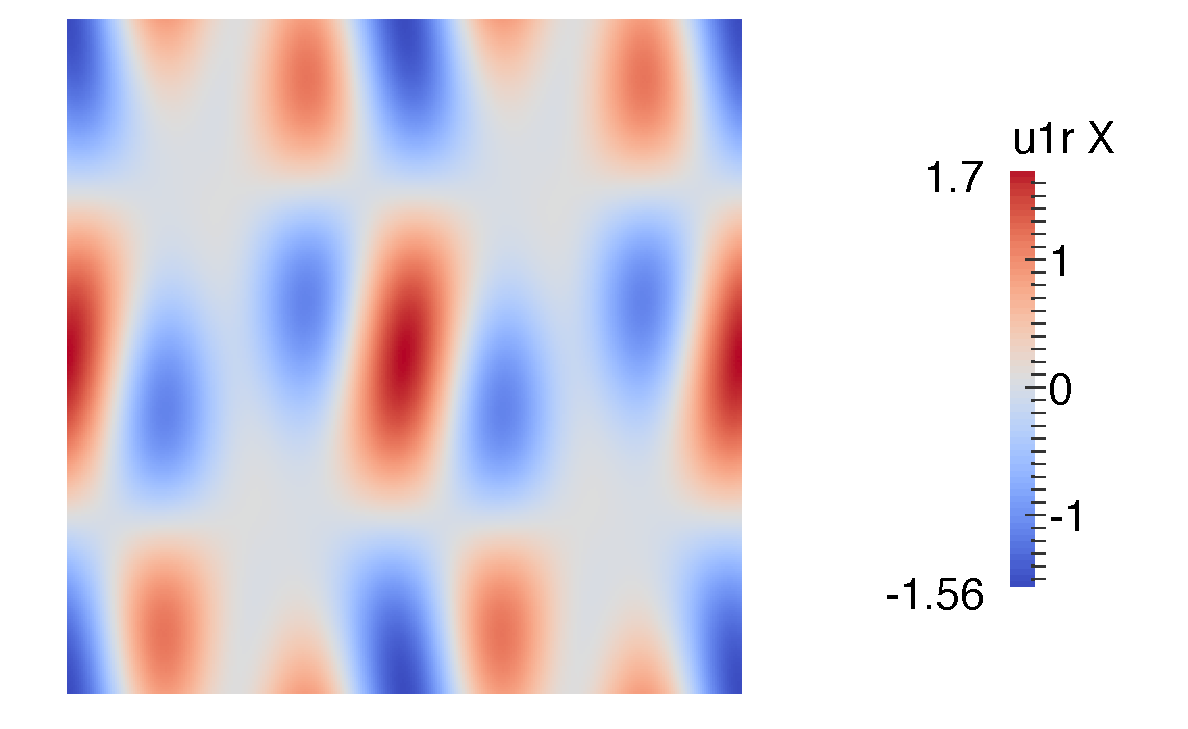
\includegraphics[width=0.45\textwidth]{results/t0.1/rexi_u}\\
  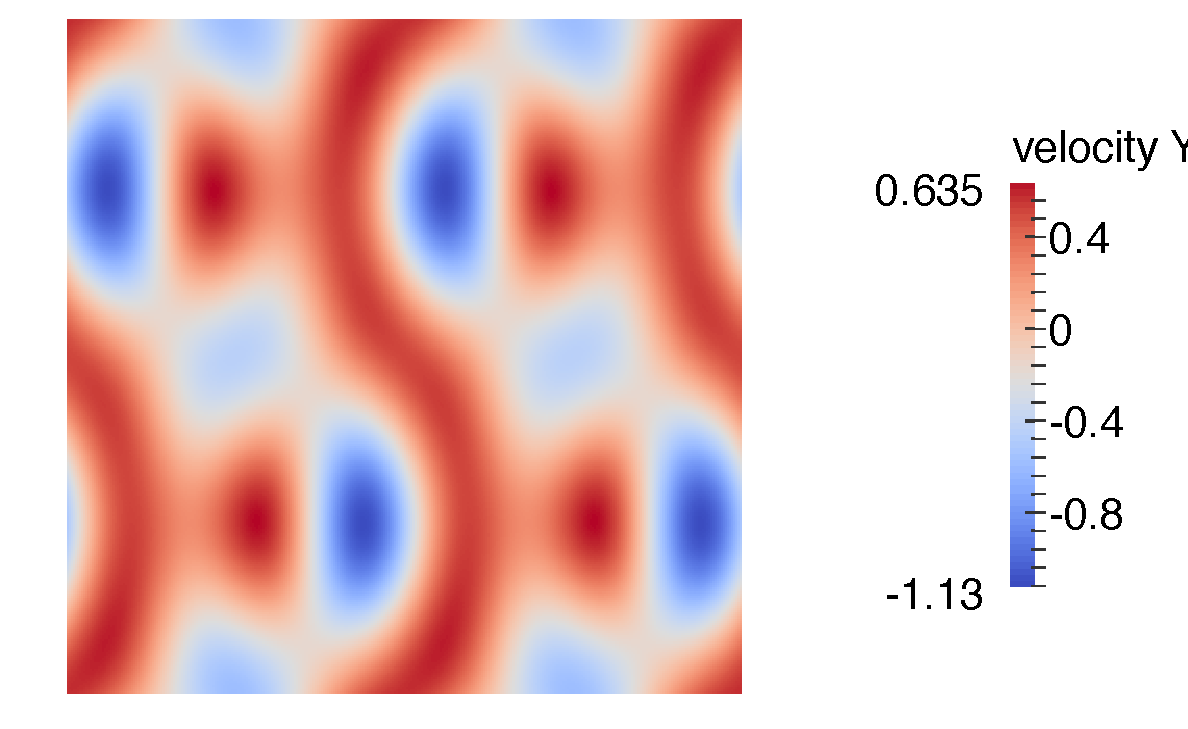
\includegraphics[width=0.45\textwidth]{results/t0.1/IM_v}
  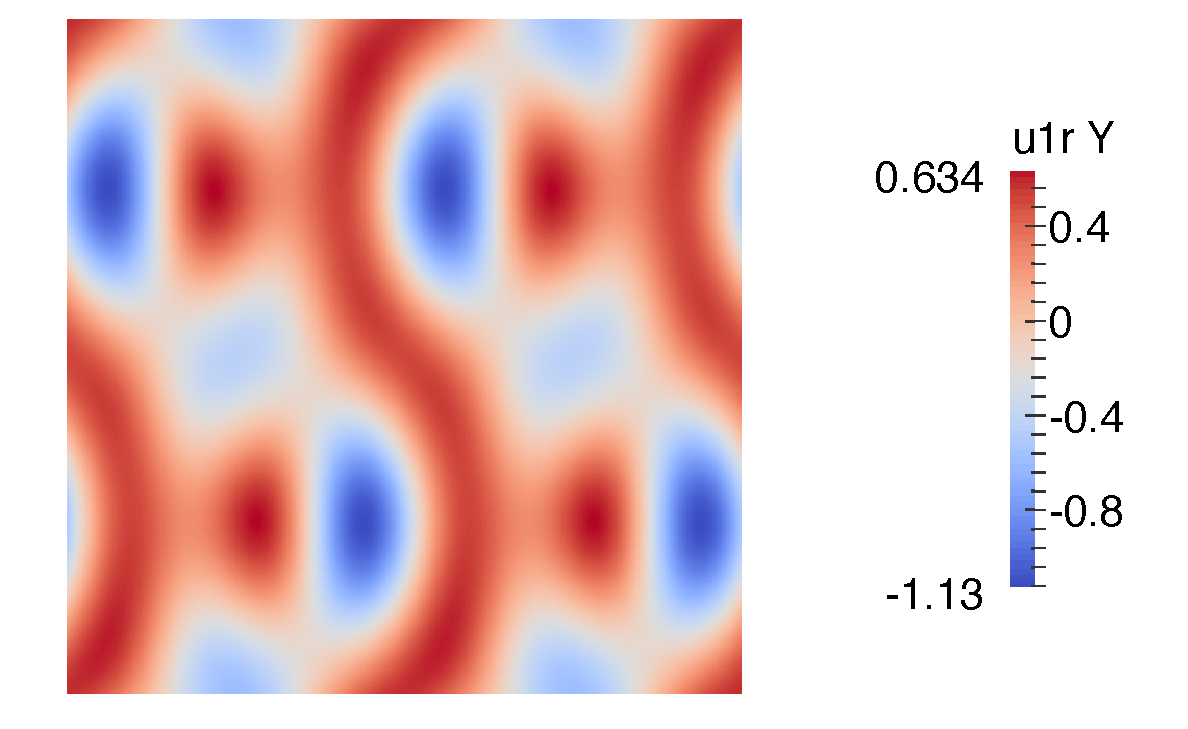
\includegraphics[width=0.45\textwidth]{results/t0.1/rexi_v}
\caption{h (top), u (middle) and v (bottom) at $t=0.1$. Implicit midpoint imestepping on the left, REXI on the right.}
\end{figure}

\end{document}
